\documentclass[10pt,a4paper]{memoir}
% Margins
\setulmarginsandblock{2.5cm}{2.5cm}{*}
\setlrmarginsandblock{2cm}{2cm}{*}
\checkandfixthelayout
% Language
\usepackage[english]{babel}
% Graphics
\usepackage[pdftex]{graphicx}
\graphicspath{{./figures/}}
\DeclareGraphicsExtensions{.pdf,.jpg,.jpeg,.png}
\usepackage{todonotes}
% Math
\usepackage[cmex10]{amsmath}
\interdisplaylinepenalty=2500{}
\usepackage{steinmetz}
% Floats
\usepackage{booktabs,multirow}
\usepackage[caption=true,font=footnotesize]{subfig}
\usepackage{wrapfig}
% Useful Macros
\newcommand{\sref}[1]{Section~\ref{#1}}
\newcommand{\code}[1]{\texttt{#1}}
\newcommand\mat[1]{\boldsymbol{#1}}
\newcommand\vect[1]{\boldsymbol{#1}}
\newcommand\matop[2]{\boldsymbol{#1}\left({#2}\right)}
% Tikz
\usepackage{tikz}
\usepackage[american,siunitx]{circuitikz}
\ctikzset{voltage/distance from node=0.8}
\newcommand*\circled[1]{\tikz[baseline=(char.base)]{
            \node[shape=circle,draw,inner sep=2pt] (char) {#1};}}
\tikzset{
    partial ellipse/.style args={#1:#2:#3}{
        insert path={+ (#1:#3) arc (#1:#2:#3)}
    }
}
\newlength\figwidth
% Exercises environment
\usepackage{exsheets}
\SetupExSheets{
  question/print = true ,
  solution/print = true ,
  counter-format = ch.qu ,
  counter-within = chapter
}
% Acronyms
\usepackage[acronym,shortcuts]{glossaries}
\glsdisablehyper
\newacronym{kcl}{KCL}{Kirchhoff's Current Law}
\newacronym{kvl}{KVL}{Kirchhoff's Voltage Law}
% Memoir customization
\makeatletter
\renewcommand\memendofchapterhook{%
  \clearpage\m@mindentafterchapter\@afterheading}
\makeatother
% Reviewing
\usepackage{color}
\usepackage{showframe}
\renewcommand{\ShowFrameColor}{\color{yellow}}
\renewcommand{\ShowFrameLinethickness}{0.1pt}


\title{MA2009: Introduction to Electrical Circuit and Electronic Devices}
\author{Francisco Su\'{a}rez-Ruiz}

\begin{document}
\maketitle

% Tutorial T1
\chapter{Circuits Fundamentals}
% T1.1
\begin{question}
  \textbf{Kirchhoff's Laws}
  \begin{figure}[!h]
    \centering
    \includegraphics[scale=1]{t01-1a}
    \caption{}
    \label{fig:t01-1a}
  \end{figure}
  \begin{enumerate}
    \item Identify loop and meshes in the circuit of \fref{fig:t01-1a}.
    \item Apply \ac{kvl} to find voltages $v_1$ and $v_2$.
  \end{enumerate}
\end{question}
\begin{solution}
  \begin{figure}[!h]
    \centering
    \includegraphics[scale=1]{t01-1b}
  \end{figure}
 \begin{enumerate}
    \item There are 3 loops and 2 meshes (only \circled{1} and \circled{2})
    \item \ac{kvl} at mesh \circled{1}:
    \begin{gather*}
      v_s - v_3 - v_2 = 0 \\
      v_2 = v_s - v_3 = \SI{5}{\volt} - \SI{3}{\volt} = \SI{2}{\volt}
    \end{gather*}
    \ac{kvl} at mesh \circled{2}:
    \begin{gather*}
      v_2 + v_4 - v_1 = 0 \\
      v_1 = v_2 + v_4  = \SI{2}{\volt} - \SI{10}{\volt} = \SI{12}{\volt}
    \end{gather*}
  \end{enumerate}
\end{solution}

% T1.2
\newpage
\begin{question}
  \begin{wrapfigure}{r}{6.5cm}
    \centering
    \includegraphics[scale=1]{t01-2a}
    \caption{}
    \label{fig:t01-2a}
  \end{wrapfigure}
  \textbf{Kirchhoff's Laws}
  \begin{enumerate}
    \item Identify all the nodes in the circuit of \fref{fig:T1-2a}. What can you say about the ground?
    \item Using \ac{kcl}, determine the current through $R_3$ knowing that:
    \begin{itemize}
      \item $v_s = \SI{12}{\volt}$
      \item $R_s = \SI{1}{\kilo\ohm}$
      \item $R_1 = \SI{2}{\kilo\ohm}$
      \item $R_2 = \SI{4}{\kilo\ohm}$
      \item $R_3 = \SI{6}{\kilo\ohm}$
    \end{itemize}
  \end{enumerate}
\end{question}
\begin{solution}
  \begin{figure}[!h]
    \centering
    \missingfigure[figwidth=6cm]{}
  \end{figure}
\end{solution}

\chapter{Solving Networks and Power}
\chapter{Node-Voltage, Mesh-Current and Superposition}
\chapter{Thevenin and Norton}
\chapter{Power Transfer and Energy Storage}

% Tutorial T6
\chapter{Frequency Response}
% T6.1
\newpage
\begin{question}
  \textbf{RMS and Average Voltages}
  \begin{figure}[!h]
    \centering
    \missingfigure[figwidth=6cm]{}
    \caption{}
  \end{figure}
\end{question}

% T6.2
\newpage
\begin{question}
  \textbf{Complex Numbers}
  \begin{figure}[!h]
    \centering
    \missingfigure[figwidth=6cm]{}
    \caption{}
  \end{figure}
\end{question}

% T6.3
\newpage
\begin{question}
  \textbf{Phasors}
  \begin{figure}[!h]
    \centering
    \missingfigure[figwidth=6cm]{}
    \caption{}
  \end{figure}
\end{question}

% T6.4
\newpage
\begin{question}
  \begin{wrapfigure}{r}{7.5cm}
    \centering
    \includegraphics[scale=1]{t06-4}
    \caption{$v_s(t)=10\cos{\left(100t\right)}$}
    \label{fig:t06-4}
  \end{wrapfigure}
  \textbf{AC Analysis}
  
  Apply AC analysis to determine $i_s(t)$ in the circuit shown in \fref{fig:t06-4} given that: $R_1 = \SI{50}{\ohm}$, $R_2 = \SI{200}{\ohm}$ and $C_3 = \SI{100}{\micro\farad}$. \textbf{Hint. Follow these steps:}
  \begin{enumerate}
    \item Identify the sinusoidal source and note the excitation frequency.
    \item Convert the source to phasor form.
    \item Represent each circuit element by its impedance.
    \item Solve the resulting phasor circuit, using appropriate network analysis tools.
    \item Convert the (phasor-form) answer to its time-domain equivalent.
  \end{enumerate}
\end{question}
\begin{solution}
  \begin{enumerate}
    \item From the sinusoidal source, $v_s(t)=10\cos{\left(100t\right)}$, the excitation frequency is $\omega=100$ $\frac{\mbox{rad}}{\mbox{s}}$.
    \item $V_s(j\omega)=10\phase{0}$ \si{\volt}.
    \item The resistors impedance has only real component in the frequency-domain. For the capacitor we need to consider the excitation frequency, therefore:
    \begin{gather*}
      Z_1 = 50 \si{\ohm}\\
      Z_2 = 200 \si{\ohm}\\
      Z_3 = \dfrac{1}{j\omega C_3} = \dfrac{1}{j 100\times100\times10^{-6}} = \dfrac{1}{j0.01} = -j100\si{\ohm}
    \end{gather*}
    \item We can calculate the current $I_s$ by simply calculating the equivalent resistance of the circuit and applying Ohm's law:
    \begin{figure}[!h]
      \centering
      \subfloat[Initial circuit]{\includegraphics[scale=1]{t06-4a}}\qquad
      \subfloat[Equivalent circuit]{\includegraphics[scale=1]{t06-4b}}
  \end{figure}
  \begin{align*}
    I_s &= \dfrac{V_s}{Z_{eq}} \\
    Z_{eq} &= Z_1 + \left( Z_2  \parallel Z_3 \right) \\
    Z_2\parallel Z_3 &= \dfrac{Z_2 Z_3}{Z_2+Z_3} = \dfrac{200(-j100)}{200 - j100} = \dfrac{-j200}{2 - j} = \dfrac{-j200}{2 - j}\times\dfrac{2 + j}{2 + j} = \dfrac{200-j400}{5} = \left( 40 - j80 \right)\si{\ohm} \\
    Z_{eq} &= 50 + \left( 40 - j80 \right) = \left( 90 - j80 \right)\si{\ohm} \\
    I_s(j\omega) &= \dfrac{10}{90 - j80} = \dfrac{1}{9 - j8}\times\dfrac{9 + j8}{9 + j8} = \dfrac{9 + j8}{145} = \left( 0.062069 + j0.055172 \right)\si{\ampere} \\
    &= \sqrt{0.062069^2 + 0.055172^2}\phase{\tan^{-1}\left(\frac{0.055172}{0.062069}\right)} = 0.083045\phase{0.72664}\si{\ampere}
  \end{align*}
  \item Converting to the time-domain:
  \begin{equation*}
    i_s(t) = 0.083045\cos{\left(100t + 0.72664\right)} \si{\ampere} 
  \end{equation*}
  \end{enumerate}
\end{solution}

% Tutorial T7
\chapter{Review}
We shall use this slot to:
\begin{itemize}
  \item Conclude any previous tutorial questions left uncovered
  \item Familiarize with an \textbf{online circuit simulator}: https://www.circuitlab.com/
  
  NOTE: Exist a NTU-wide license, you must sign-up with your official NTU email account.
  \item Familiarize with an \textbf{online calculator}: https://octave.im/
\end{itemize}

% Tutorial T8
\chapter{Passive Filters}

% T8.1
\begin{question}
  \begin{wrapfigure}{r}{8cm}
    \centering
    \includegraphics[scale=1]{t08-1a}
    \caption{}
    \label{fig:t08-1a}
  \end{wrapfigure}
  \textbf{Cut-off Frequency}
  
  In the circuit shown in \fref{fig:t08-1a}, find the expression of the frequency response $H$ and plot the corresponding Bode plot for $R_1=\SI{1}{\ohm}$, $R_2=\SI{2}{\ohm}$ and $C=\SI{1}{\micro\farad}$.
  \begin{enumerate}
    \item Is it a high-pass or low-pass filter?
    \item What is the gain in the pass-band?
    \item Find the $-3\si{dB}$
  \end{enumerate}
\end{question}
\begin{solution}
  Solution goes here
\end{solution}

% T8.2
\newpage
\begin{question}
  \textbf{RLC Filters}
  
  For each of the filters shown in \fref{fig:t08-2} find, without writing the complete frequency response, a simple expression for the frequency response when the frequency is very low ($\omega\to 0$) and when it is very high ($\omega\to\infty$). Are they filter low-pass or high-pass?
  \begin{figure}[!h]
    \centering
    \subfloat[]{\includegraphics[scale=1]{t08-2a}} \qquad\qquad
    \subfloat[]{\includegraphics[scale=1]{t08-2b}} \\
    \subfloat[]{\includegraphics[scale=1]{t08-2c}} \qquad\qquad
    \subfloat[]{\includegraphics[scale=1]{t08-2d}}
    \caption{}
    \label{fig:t08-2}
  \end{figure}
\end{question}
\begin{solution}
  Solution goes here
\end{solution}

% Tutorial T9
\chapter{Diodes}

% Tutorial T10
\chapter{Transistors and Amplification}

% T10.1
\begin{question}
  For each transistor shown in \fref{fig:t10-1}, determine the operating region. Assume $V_{\gamma}=\SI{0.6}{\volt}$.
  \begin{figure}[!h]
    \centering
    \subfloat[]{\includegraphics[scale=1]{t10-1a}} \qquad\qquad
    \subfloat[]{\includegraphics[scale=1]{t10-1b}} \qquad\qquad
    \subfloat[]{\includegraphics[scale=1]{t10-1c}}
    \caption{}
    \label{fig:t10-1}
  \end{figure}
\end{question}
\begin{solution}
  \begin{table}[!h]
  \centering
  \begin{tabular}{l | l l}
    \toprule
     & $V_{CE} \leq V_{\gamma}$ & $V_{CE} > V_{\gamma}$ \\
    \midrule
    $V_{BE} < V_{\gamma}$     & Cut-off     & Cut-off \\
    $V_{BE} \geq V_{\gamma}$  & Saturation  & Active \\
    \bottomrule
  \end{tabular}
  \caption{Operation regions of a BJT}
  \end{table}
  \begin{enumerate}[(a)]
    \item This is a \textbf{npn} transistor.
      \begin{equation*}
        \left.
        \begin{aligned}
          V_{BE} = \SI{0.7}{\volt} \, &> V_{\gamma} \\
          V_{CE} = \SI{0.3}{\volt} \, &< V_{\gamma}
        \end{aligned} \right\rbrace \implies \mbox{BJT is in the \textbf{saturation} region.}
      \end{equation*}
    \item This is a \textbf{npn} transistor.
      \begin{gather*}
        V_{CE} = \SI{0.2}{\volt} \\
        V_{CB} = \SI{0.7}{\volt} \\
        V_{CE} = V_{CB} + V_{BE} \implies V_{BE} = V_{CE} - V_{CB} = 0.2 - 0.7 =  -\SI{0.5}{\volt} \\
        \left.
        \begin{aligned}
          V_{BE} = -\SI{0.5}{\volt} \, &< V_{\gamma} \\
          V_{CE} =  \SI{0.2}{\volt} \, &< V_{\gamma}
        \end{aligned} \right\rbrace \implies \mbox{BJT is in the \textbf{cut-off} region.}
      \end{gather*}
    \item This is a \textbf{npn} transistor.
    \begin{gather*}
        V_{CB} = \SI{5.4}{\volt} \\
        V_{BE} = \SI{0.7}{\volt} \\
        V_{CE} = V_{CB} + V_{BE} = 5.4 - 0.7 =  \SI{6.1}{\volt} \\
        \left.
        \begin{aligned}
          V_{BE} = \SI{0.7}{\volt} \, &> V_{\gamma} \\
          V_{CE} = \SI{6.1}{\volt} \, &> V_{\gamma}
        \end{aligned} \right\rbrace \implies \mbox{BJT is in the \textbf{active} region.}
      \end{gather*}
  \end{enumerate}
\end{solution}

% T10.2
\newpage
\begin{question}
  The transistor 2N3904, which has given I-V curve shown in \fref{fig:t10-2a}, is now connected in the circuit shown in \fref{fig:t10-2b}. Derive the load line equation and graphically determine the Q-point of the transistor.
  \begin{figure}[!h]
    \centering
    \subfloat[]{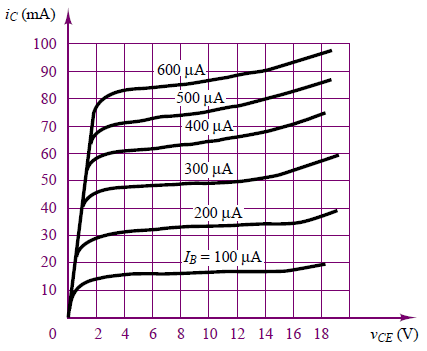
\includegraphics[height=50mm]{bjt-i-v-curve}\label{fig:t10-2a}} \qquad\qquad
    \subfloat[]{\includegraphics[height=50mm]{t10-2b}\label{fig:t10-2b}}
    \caption{}
  \end{figure}
\end{question}
\begin{solution}
  \setlength\figwidth{80mm}
  \begin{wrapfigure}{r}{8cm}
    \centering
    \begin{tikzpicture}
      \node[draw=none,fill=none,anchor=south west,inner sep=0] at (0,0) {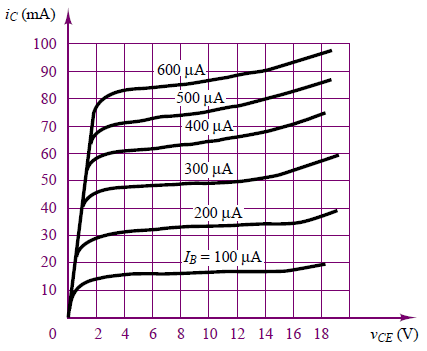
\includegraphics[width=\figwidth]{bjt-i-v-curve}};
      \node[circle,fill=red,inner sep=0pt,minimum size=0.025\figwidth] (P1) at (0.157\figwidth,0.725\figwidth) {};
      \node[circle,fill=red,inner sep=0pt,minimum size=0.025\figwidth] (P2) at (0.825\figwidth,0.075\figwidth) {};
      \draw[red,very thick] (P1) edge (P2);
      \node[circle,fill=blue,inner sep=0pt,minimum size=0.025\figwidth] (I) at (0.6\figwidth,0.295\figwidth) {};
      \node[inner sep=0pt] (X) at (0.6\figwidth,0.075\figwidth) {};
      \node[inner sep=0pt] (Y) at (0.157\figwidth,0.295\figwidth) {};
      \draw[blue,thick,dashed] (X) edge (I);
      \draw[blue,thick,dashed] (Y) edge (I);
    \end{tikzpicture}
  \end{wrapfigure}
  Let's assume that the transistor in the \textbf{active} region.
  \newline
  Applying KVL at mesh \circled{1}:
  \begin{gather*}
    V_{cc} - I_{C}R_{c} - V_{CE} = 0 \\
    I_{C} = \dfrac{V_{cc} - V_{CE}}{R_{c}} \\
    I_{C}\left(V_{CE}\right) = \dfrac{20 - V_{CE}}{200}\implies \mbox{Load-line equation} \\
  \end{gather*}
  We select 2 points to plot the line on top of the transistor's I-V curve.
  \begin{gather*}
    \mbox{If}\quad V_{CE}=0 \\
    I_{c}(0) = \dfrac{20 - 0}{200} = \SI{100}{\milli\ampere} \implies P_1 = \left( 0, 100\right) \\
    \mbox{If}\quad I_{C}=0 \\
    0 = \dfrac{20 - V_{CE}}{200} \implies V_{CE} = \SI{20}{\volt} \implies P_2 = \left( 20, 0\right)
  \end{gather*}
  \newline
  The Q-point of the circuit if defined as:
  \begin{equation*}
    I_{BQ} = \SI{200}{\micro\ampere} \qquad;\qquad I_{CQ}\approx \SI{33}{\milli\ampere} \qquad;\qquad V_{CE} \approx \SI{13.5}{\volt}
  \end{equation*}
\end{solution}

% T10.3
\newpage
\begin{question}
  \begin{wrapfigure}{r}{6.5cm}
    \centering
    \includegraphics[scale=0.8]{t10-3}
    \caption{}
    \label{fig:t10-3}
  \end{wrapfigure}
  Given the circuit of \fref{fig:t10-3}, determine the operation point of the transistor. Assume a $\SI{0.6}{\volt}$ offset voltage and $\beta = 150$. In what region is the transistor?
\end{question}
\begin{solution}
  Solution goes here
\end{solution}

% T10.4
\newpage
\begin{question}
THe circuit is a common-collector
\end{question}
\begin{solution}
  Solution goes here
\end{solution}

% T10.5
\newpage
\begin{question}
  \begin{wrapfigure}{r}{7cm}
    \centering
    \includegraphics[scale=0.75]{t10-5}
    \caption{}
    \label{fig:t10-5}
  \end{wrapfigure}
  Given the circuit of \fref{fig:t10-5}, determine the operation point (Q-point) of the transistor. Assume a $\SI{0.7}{\volt}$ offset voltage and $\beta = 100$. In what region is the transistor?
  \begin{align*}
    V_{BB} &= \SI{6}{\volt}      & V_{CC}  &= \SI{12}{\volt}     \\
    R_{B} &= \SI{10}{\kilo\ohm} & R_{C}   &= \SI{10}{\kilo\ohm} \\
    R_{E} &= \SI{2}{\kilo\ohm}  & 
  \end{align*}
  
\end{question}
\begin{solution}
  Let's assume that the transistor is in the \textbf{active} region, therefore,
  \begin{flalign*}
    V_{BE} &= V_{\gamma} =  \SI{0.7}{\volt} &\\
    I_{C}  &= \beta I_{B} &\\
    I_{E}  &= I_{B} + I_{C} = \left( \beta+1 \right) I_{B} &
  \end{flalign*}
  KVL at mesh \circled{1}:
  \begin{gather*}
    V_{BB} - I_{B}R_{B} - V_{BE} - I_{E}R_{E} = 0 \\
    V_{BB} - I_{B}R_{B} - V_{BE} - \left( \beta+1 \right) I_{B}R_{E} = 0 \\
    I_{B} = \dfrac{V_{BB} - V_{BE}}{R_{B} + \left( \beta+1 \right) R_{E}} = \SI{25}{\micro\ampere}
  \end{gather*}
  KVL at mesh \circled{2}:
  \begin{gather*}
    V_{CC} - I_{C}R_{C} - V_{CE} - I_{E}R_{E} = 0 \\
    V_{CC} - \beta I_{B}R_{C} - V_{CE} - \left( \beta+1 \right) I_{B}R_{E} = 0 \\
    V_{CE} = V_{CC} - I_{B}\left[ \beta R_{C} - \left(\beta+1\right)R_{E}\right] = \SI{-7.95}{\volt}
  \end{gather*}
  Given that $V_{CE} = \SI{-7.95}{\volt} < V{\gamma}$, our assumption was \text{wrong}. The transistor is \textbf{not active}.
  
  \bigskip
  \textbf{IMPORTANT:} The following is included just for reference and can be skipped. If you check in the lectures, the Q-point is discussed only for active transistors.
  
  \bigskip
  \bigskip
  Now, let's assume that the transistor is in the \textbf{saturation} region. Typical saturation values are around $V_{sat} = \SI{0.2}{\volt}$, therefore,
  \begin{gather*}
    V_{BE} = V_{\gamma} =  \SI{0.7}{\volt}  \\
    V_{CE} = V_{sat} = \SI{0.2}{\volt}      \\
    I_{E}  = I_{B} + I_{C}
  \end{gather*}
  Now that we know $V_{CE}$, the circuit can be solved using node voltage method and Ohm's law,
  \begin{equation*}
    I_B = \dfrac{V_{BB} - V_B}{R_B}  \qquad\qquad I_C = \dfrac{V_{CC} - V_C}{R_C} \qquad\qquad I_E = \dfrac{V_E}{R_E}
  \end{equation*}
  \begin{align}
    I_E &= I_B + I_C \nonumber \\
    \dfrac{V_E}{R_E} &= \dfrac{V_{BB} - V_B}{R_B} - \dfrac{V_{CC} - V_C}{R_C} \label{eq:t10-5a} \\
    V_{CE} &= V_C - V_E \implies V_C = V_{CE} + V_E \label{eq:t10-5b} \\
    V_{BE} &= V_B - V_E \implies V_B = V_{BE} + V_E \label{eq:t10-5c} 
  \end{align}
  Replacing \eqref{eq:t10-5b} and \eqref{eq:t10-5c} into \eqref{eq:t10-5a},
  \begin{align*}
    \dfrac{V_E}{R_E} &= \dfrac{V_{BB} - V_{BE} - V_E}{R_B} - \dfrac{V_{CC} - V_{CE} - V_E}{R_C} \\
    V_E\left(\dfrac{1}{R_B} + \dfrac{1}{R_C} + \dfrac{1}{R_E}\right) &= \dfrac{V_{BB} - V_{BE}}{R_B} + \dfrac{V_{CC} - V_{CE}}{R_C} \implies V_E = \SI{3.607}{\volt}
  \end{align*}
  Once we know the value of $V_E$, it's possible to determine the operating point of the transistor,
  \begin{align*}
    V_B &= V_{BE} + V_E = \SI{4.307}{\volt} \\
    V_C &= V_{CE} + V_E = \SI{3.807}{\volt} \\
    I_{BQ} &= \dfrac{V_{BB} - V_B}{R_B} = \SI{169.2}{\micro\ampere} \\
    I_{CQ} &= \dfrac{V_{CC} - V_C}{R_C} = \SI{819.3}{\micro\ampere} \\
    V_{CEQ} &= V_{sat} = \SI{0.2}{\volt}
  \end{align*}
\end{solution}

\end{document}
